% !TeX root = ../main.tex
% Add the above to each chapter to make compiling the PDF easier in some editors.

\chapter{Heatmaps}\label{chapter:Heatmaps}

In diesem Kapitel werden Heatmaps der Feintypen 211, 224, 243, 244, 623, 631, 641 und 651 dargestellt. Anhand der Heatmaps können Bereiche oder Punkte innerhalb des Testgebiets ausfindig gemacht werden, in bzw. an denen es besonders häufig zu Unfällen mit den oben genannten Feintypen kam. Alle Heatmaps der Feintypen, denen die Risiko-Kategorie \textit{c} oder \textit{d} zugeordnet wurde sind als html-Datei auf der angehängten CD zu finden. Die Darstellung in einer interaktiven Karte ermöglicht es, auffällige Stellen durch Vergrößern genauer zu betrachten.

\begin{savenotes}
	\begin{figure}[H]
		\centering
		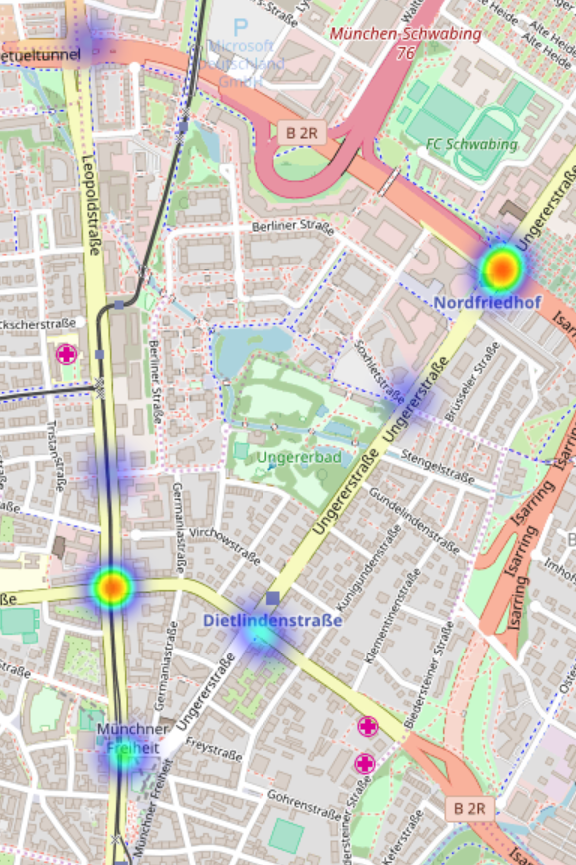
\includegraphics[width=6cm,height=9cm]{figures/HM_211}
		\caption[Heatmap der Unfälle mit dem Feintyp 211]{Heatmap der Unfälle mit dem Feintyp 211}\label{fig:Heatmap_211}
	\end{figure}
\end{savenotes}

\begin{savenotes}
	\begin{figure}[H]
		\centering
		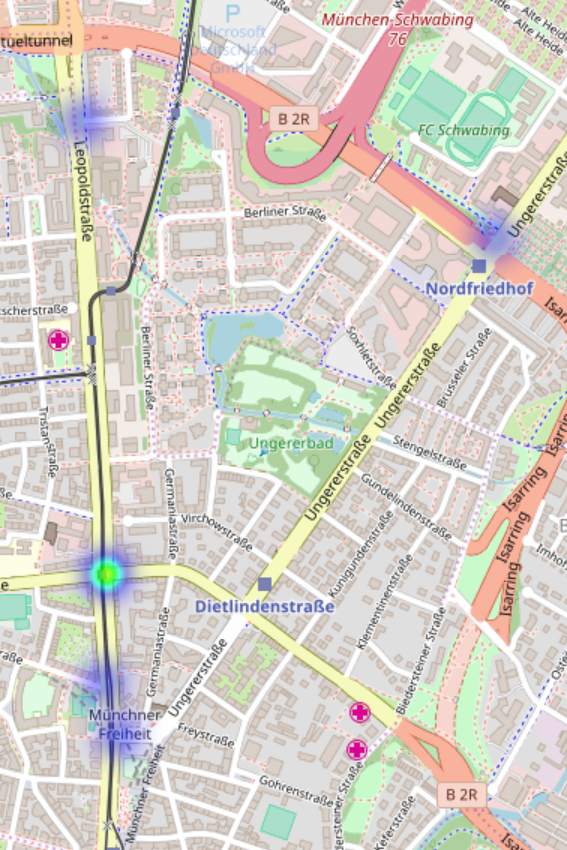
\includegraphics[width=6cm,height=9cm]{figures/HM_224}
		\caption[Heatmap der Unfälle mit dem Feintyp 224]{Heatmap der Unfälle mit dem Feintyp 224}\label{fig:Heatmap_224}
	\end{figure}
\end{savenotes}

\begin{savenotes}
	\begin{figure}[H]
		\centering
		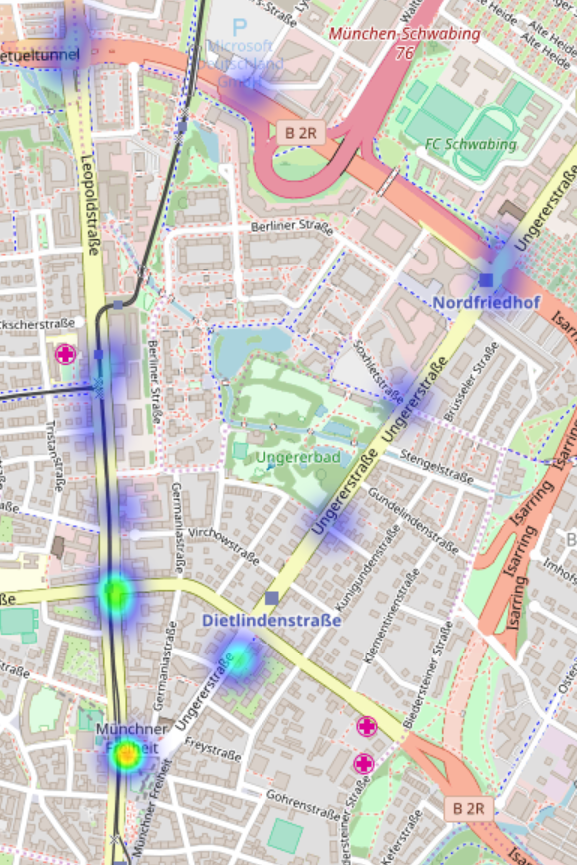
\includegraphics[width=6cm,height=9cm]{figures/HM_243}
		\caption[Heatmap der Unfälle mit dem Feintyp 243]{Heatmap der Unfälle mit dem Feintyp 243}\label{fig:Heatmap_243}
	\end{figure}
\end{savenotes}

\begin{savenotes}
	\begin{figure}[H]
		\centering
		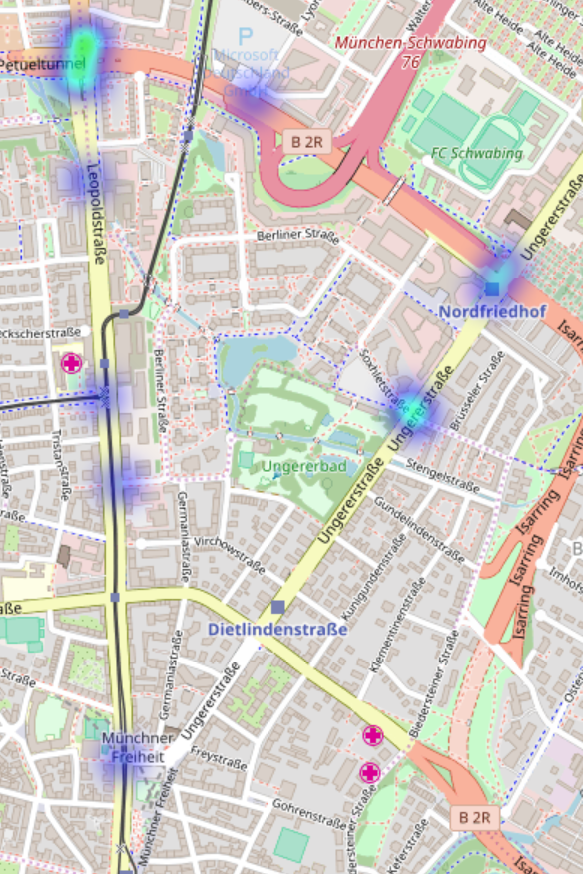
\includegraphics[width=6cm,height=9cm]{figures/HM_244}
		\caption[Heatmap der Unfälle mit dem Feintyp 244]{Heatmap der Unfälle mit dem Feintyp 244}\label{fig:Heatmap_244}
	\end{figure}
\end{savenotes}

\begin{savenotes}
	\begin{figure}[H]
		\centering
		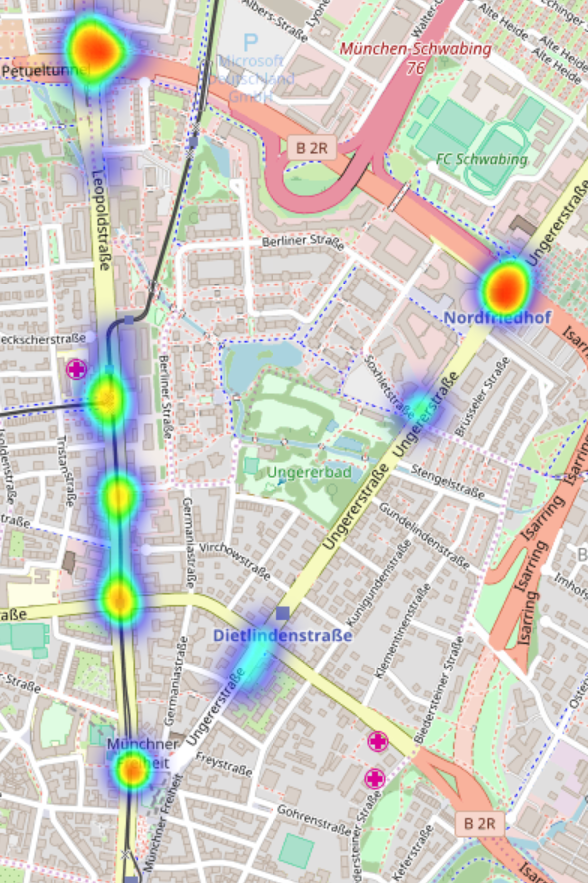
\includegraphics[width=6cm,height=9cm]{figures/HM_623}
		\caption[Heatmap der Unfälle mit dem Feintyp 623]{Heatmap der Unfälle mit dem Feintyp 623}\label{fig:Heatmap_623}
	\end{figure}
\end{savenotes}

\begin{savenotes}
	\begin{figure}[H]
		\centering
		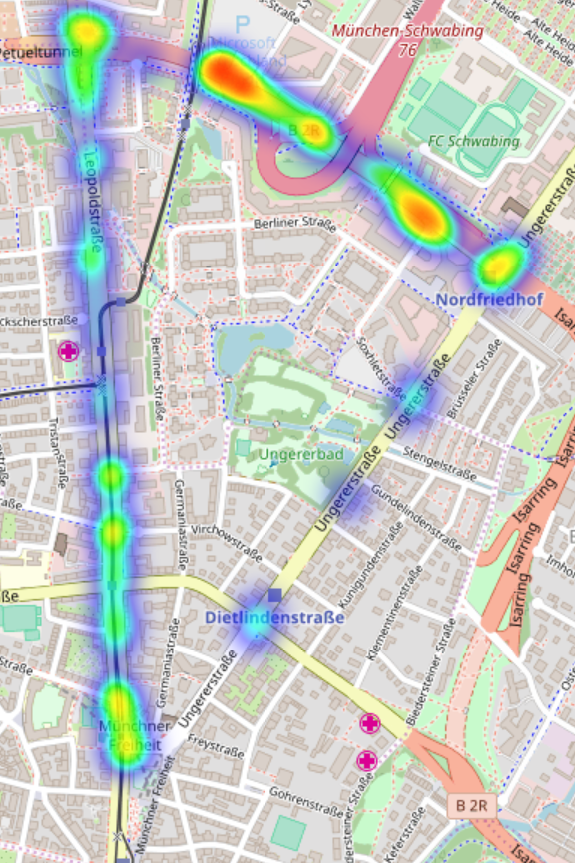
\includegraphics[width=6cm,height=9cm]{figures/HM_631}
		\caption[Heatmap der Unfälle mit dem Feintyp 631]{Heatmap der Unfälle mit dem Feintyp 631}\label{fig:Heatmap_631}
	\end{figure}
\end{savenotes}

\begin{savenotes}
	\begin{figure}[H]
		\centering
		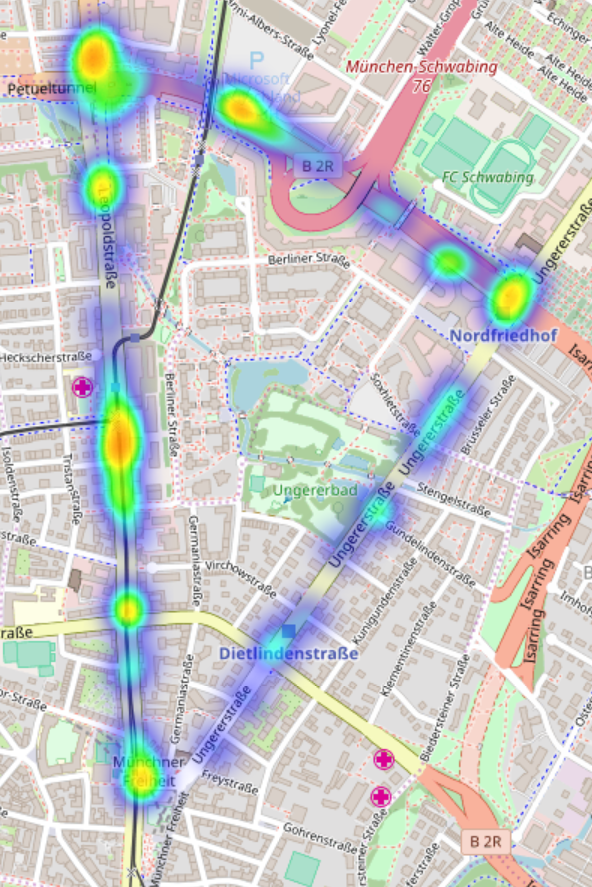
\includegraphics[width=6cm,height=9cm]{figures/HM_641}
		\caption[Heatmap der Unfälle mit dem Feintyp 641]{Heatmap der Unfälle mit dem Feintyp 641}\label{fig:Heatmap_641}
	\end{figure}
\end{savenotes}

\begin{savenotes}
	\begin{figure}[H]
		\centering
		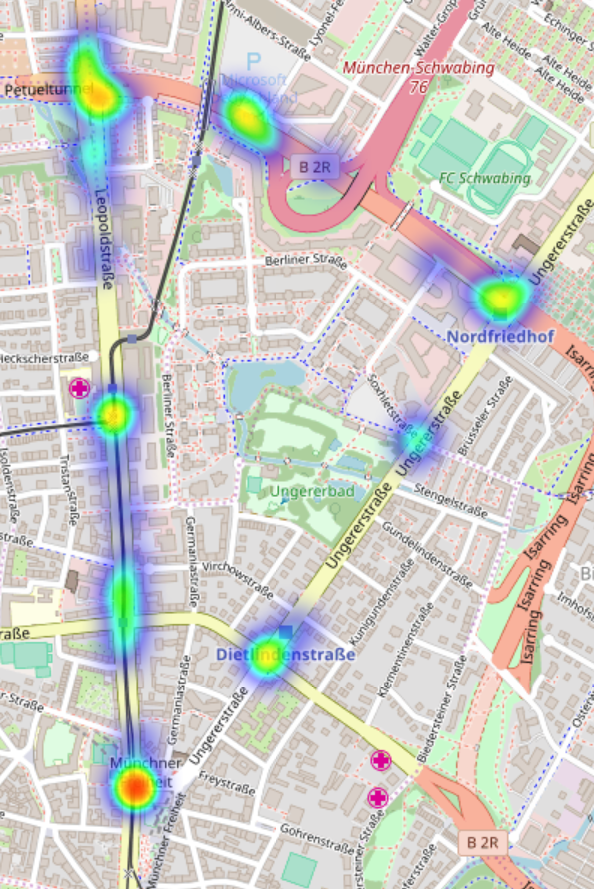
\includegraphics[width=6cm,height=9cm]{figures/HM_651}
		\caption[Heatmap der Unfälle mit dem Feintyp 651]{Heatmap der Unfälle mit dem Feintyp 651}\label{fig:Heatmap_651}
	\end{figure}
\end{savenotes}